\documentclass{beamer}
%
% Choose how your presentation looks.
%
% For more themes, color themes and font themes, see:
% http://deic.uab.es/~iblanes/beamer_gallery/index_by_theme.html
%
\mode<presentation>
{
  \usetheme{default}      % or try Darmstadt, Madrid, Warsaw, ...
  \usecolortheme{default} % or try albatross, beaver, crane, ...
  \usefonttheme{default}  % or try serif, structurebold, ...
  \setbeamertemplate{navigation symbols}{}
  \setbeamertemplate{caption}[numbered]
} 
\usepackage{sansmathaccent}
\usepackage{xmpmulti}
\pdfmapfile{+sansmathaccent.map}
\usepackage[english]{babel}
\usepackage[utf8x]{inputenc}
\usepackage{multimedia}
\usepackage{graphicx}
\usepackage{multimedia}
\usepackage{tikz}
\usepackage{subcaption}
%\usepackage{animate}
\title[Your Short Title]{Exploration of chaos in shock waves}
\author{Jithin D. George}
%\institute{Where You're From}
%\date{Date of Presentation}
\AtBeginSection[]{\frame{\frametitle{Outline}%
		\usebeamerfont{myTOC}\tableofcontents[current]}}
\begin{document}

\begin{frame}
  \titlepage
\end{frame}

% Uncomment these lines for an automatically generated outline.
%\begin{frame}{Outline}
%  \tableofcontents
%\end{frame}

\section{Introduction}

\subsection{Background}
\begin{frame}{Background: Reactive Euler equations and detonation }

	\[\frac{D\rho}{Dt}=-\rho \nabla . u\]
	\[\rho\frac{Du}{Dt}=- \nabla P\]
	\[\rho\frac{D}{Dt}\bigg(h+\frac{|u|^2}{2}\bigg)=\frac{\partial P}{\partial t}\]
	\[\frac{DY_i}{Dt}=\dot{\omega_i}\]
	  \begin{center}
	  	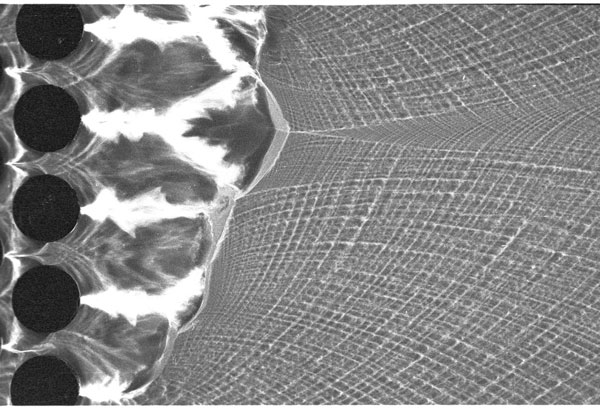
\includegraphics[height=100pt]{detonation}\\
	  	
	  \end{center}
\end{frame}	
\subsection{Model Equation}
\begin{frame}{Model Equation}


  \[u_t +\frac{1}{2}(u^2-uu_s)_x =f(x,u_s) \]

    \[x\in (-\infty,0)\]
    \[\textbf{Characteristic speed } = u-\frac{u_s}{2}\]

  






\end{frame}




	
\subsection{The nature of the source term}
\begin{frame}{The nature of the source term}
	\[f(x,u_{s})= \frac{q}{2\sqrt{4\pi \beta}} e^{-\frac{[x-x_f(u_s)]^2}{4\beta}}\]
	\[x_f(u_s) = \bigg(\frac{u_{0s}}{u_{s}}\bigg)^\alpha\]

  \begin{center}
  	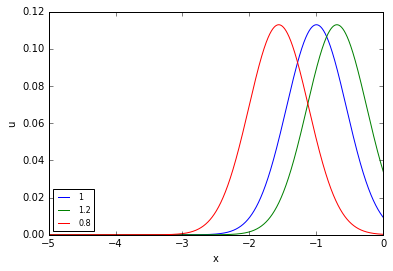
\includegraphics[height=150pt]{shiftinit}\\
  	
  \end{center}

\end{frame}	

\subsection{The steady state solution (The fixed point of a pde)}
\begin{frame}{The steady state solution (The fixed point of a pde)}
	
	
	\[\frac{1}{2}(u_0^2-u_0u_{0s})' =f(x,u_{0s}) \]
	
	\[u_0(x)=\frac{u_{0s}}{2}+ \sqrt{2\int_{-\infty}^{x}f(y,u_{0s})dy}\]
	\[f= \frac{q}{2\sqrt{4\pi \beta}} e^{-\frac{[x-x_f(u_s)]^2}{4\beta}}\]
	\[u_0(x)= \frac{1}{2}\bigg[1+ \sqrt{\frac{1+erf((x+1)/2\sqrt{\beta})}{1+erf(1/2\sqrt{\beta})}}\bigg]\]
	
\end{frame}
	
\subsection{Effects of $\beta$}
\begin{frame}{Effects of $\beta$}
\begin{figure}[H]
	\centering
	\begin{subfigure}{.5\textwidth}
		\centering
		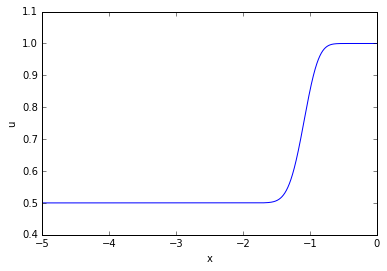
\includegraphics[width=\linewidth]{beta01}
		\caption{$\beta$ =0.01}
		\label{fig:sub1}
	\end{subfigure}%
	\begin{subfigure}{.5\textwidth}
		\centering
		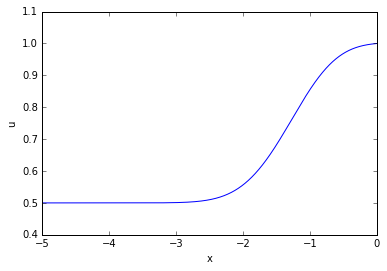
\includegraphics[width=\linewidth]{beta1}
		\caption{$\beta$ =0.1}
		\label{fig:sub2}
	\end{subfigure}
	\caption{$u_0$ for various values of $\beta$}
\end{figure}
\href{https://www.youtube.com/watch?v=nmbc-g3oGao}{Movie}	
\end{frame}	
\subsection{Numerical setup}
\begin{frame}{Numerical setup}
	\begin{itemize}
		\item \[u_t +\frac{1}{2}(u^2-uu_s)_x =a e^{-\frac{(x+us^{-\alpha})^2}{4\beta}} \]
		\item \[x\in (-10,0)\]
		\item Outflow boundary conditions
		\item Godunov splitting
		\item Lax-Wendroff fluxes with MC limiters 
	\end{itemize}
    
	
\end{frame}	


\section{Behaviour}
\begin{frame}{$\alpha = 2$}
	\begin{figure}[h!]
\href{https://www.youtube.com/watch?v=E4f0I4teyIc}{Movie}
	\end{figure} 
\end{frame}
\subsection{$\alpha = 2$}
\begin{frame}{Behaviour of $u_s$}
	\begin{center}
		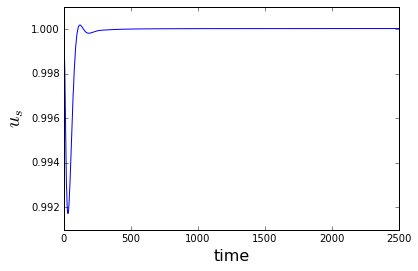
\includegraphics[height=200pt]{2}\\
		
	\end{center}	
\end{frame}


\subsection{$\alpha = 3$}
\begin{frame}{$\alpha = 3$}
	\begin{figure}[h!]
		\href{https://www.youtube.com/watch?v=E4f0I4teyIc}{Movie}
	\end{figure} 
\end{frame}
\begin{frame}{Behaviour of $u_s$}
	\begin{center}
		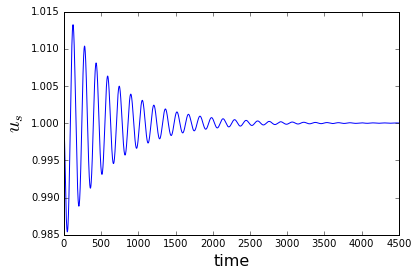
\includegraphics[height=200pt]{3b}\\
		
	\end{center}	
\end{frame}

\subsection{$\alpha = 4.6$}
\begin{frame}{$\alpha = 4.6$}
	\begin{figure}[h!]
\href{https://www.youtube.com/watch?v=iHq0bfq4zdk}{Movie} 
	\end{figure} 
\end{frame}
\begin{frame}{Asymptotic behaviour of $u_s$}
	\begin{center}
		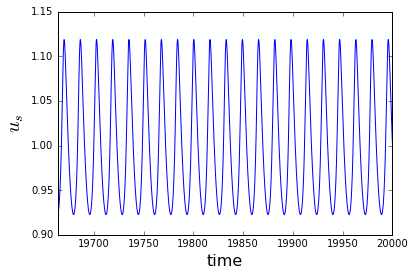
\includegraphics[height=200pt]{46}\\
		
	\end{center}	
\end{frame}
\begin{frame}{Limit cycle}
	\begin{center}
		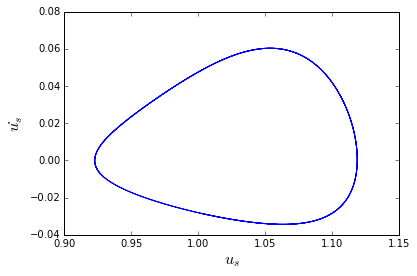
\includegraphics[height=200pt]{lim46}\\
		
	\end{center}	
\end{frame}
\subsection{$\alpha = 4.85$}
\begin{frame}{$\alpha = 4.85$}
\href{https://www.youtube.com/watch?v=0V0PySj1DOE}{Movie} 
\end{frame}
\begin{frame}{Asymptotic behaviour of $u_s$}
  \begin{center}
  	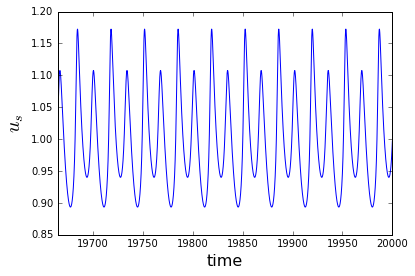
\includegraphics[height=200pt]{485}\\
  	
  \end{center}	
\end{frame}
\begin{frame}{Limit cycle}
	\begin{center}
		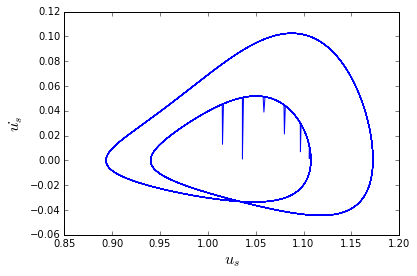
\includegraphics[height=200pt]{lim485}\\
		
	\end{center}	
\end{frame}
\subsection{$\alpha = 5.1$}
\begin{frame}{$\alpha = 5.1$}
	\begin{figure}[h!]
\href{https://www.youtube.com/watch?v=BFadoM801yg}{Movie} 
	\end{figure} 
\end{frame}
\begin{frame}{Asymptotic behaviour of $u_s$}
	\begin{center}
		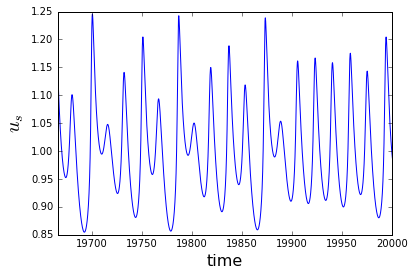
\includegraphics[height=200pt]{51}\\
		
	\end{center}	
\end{frame}
\begin{frame}{Limit cycle}
	\begin{center}
		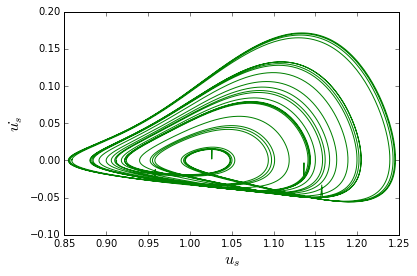
\includegraphics[height=200pt]{lim51}\\
		
	\end{center}	
\end{frame}
\section{Conclusions}

\subsection{Bifurcation diagram}
\begin{frame}{Bifurcation diagram}
	\begin{center}
		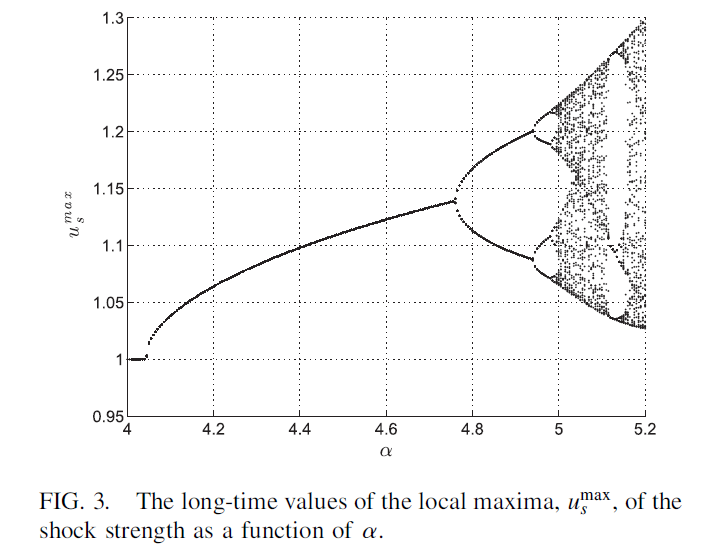
\includegraphics[height=200pt]{map}\\
		
	\end{center}	
\end{frame}
\subsection{LLE}
\begin{frame}{Largest Lyapunov Exponents}
\begin{center}
	\begin{tabular}{ | l | l | l | l |l |}
		\hline
		 & 4.85 & 4.96 & 4.97 & 5.1 \\ \hline
		LLE & 0 & 0 & 0.0042 & 0.0315\\ \hline
		$D_C$ & 1.0006 & 1.002 & 1.67 & 1.91   \\
		\hline
	\end{tabular}
\end{center}
\end{frame}
\subsection{Weird pdes and insights}
\begin{frame}{Weird pdes and insights}
	\begin{figure}[h!]
		\href{https://www.youtube.com/watch?v=RdKBWDUVpls}{Movie} 
	\end{figure} 
\end{frame}
\begin{frame}{Resources}
	\begin{itemize}
		\item Kasimov, Aslan R., Luiz M. Faria, and Rodolfo R. Rosales. "Model for shock wave chaos." Physical review letters 110.10 (2013): 104104.
		\item Faria, Luiz M., Aslan R. Kasimov, and Rodolfo R. Rosales. "Study of a model equation in detonation theory." SIAM Journal on Applied Mathematics 74.2 (2014): 547-570.

		\item \url{https://github.com/Dirivian/apps_detonation} 
	\end{itemize}	
\end{frame}
\begin{frame}{}
	\begin{center}
		
\includegraphics[height=200pt]{KASIMOV}\\
		
	\end{center}	
\end{frame}
\end{document}